%% \section{On optimal policies for selection}



%% Define selection problem and metalevel MDP representation.

%% \note{Unsure about terminology here: selection problems, sampling problems, 
%% metalevel probability model, metalevel decision problem (conflicts with Markov decision process?).}

%% ============================
\subsection{Selection problems}
%% ============================

\note{Formal definition of selection problems and the metalevel MDP with cost per sample (time value); also mention budgeted learning.}

In a \term{selection problem} the decision maker is faced with the choice between
$k$ alternative actions.  To make this choice, they may gather evidence about the
utility of each of these alternative, at some cost.  What the decision maker can know
and what they can find out is formalized in:

\begin{dfn} \label{dfn:metalevel-model}
	A \term{metalevel probability model} is a tuple $M=(U_1,\dots,U_k,\Evidence)$ 
	consisting of jointly distributed random variables:
	\begin{itemize}
		\item Real random variables $U_1,\dots,U_k$, where $U_i$ is the utility of performing action~$i$, and
		\item A countable set $\Evidence$ of random variables, each variable $E\in\Evidence$ being 
		      a computation that can be performed and whose value is the result of that computation.
	\end{itemize}
\end{dfn}
%% Not actually true that we necessarily define this with U's as roots:  in sampling models they are naturally /leaves/.

A metalevel probability model, when combined with a cost $c>0$ of computation,%
\footnote{The assumption of a fixed cost of computation is a simplification; 
	precise conditions for its validity are given by \citep{Harada:1997}.} 
defines a metalevel decision problem: what is the optimal strategy with which to choose a sequence 
of computations $E\in\Evidence$ to observe in order to maximize the expected utility 
of the action finally taken less the cost of computation?  Intuitively, 
this strategy should observe the variables which give the most evidence relevant
to deciding which action to perform, stopping when the cost of computation 
outweighs the benefit gained.

\begin{example}[Bernoulli sampling]\label{example:bernoulli}
One simple metalevel probability model is used as a model of the results of simulations \cite{someone}.
Each action will either succeed or not $U_i\in\{0,1\}$, with an unknown latent frequency of success $\Theta_i$, 
and stochastic simulations of possible consequences $E_{ij}$ can be performed:
\begin{align*}
	\Theta_i &\iid {\rm Uniform}[0,1]                      &&\quad\text{for $i=1,\dots,k$}\\
	U_i \given \Theta_i &\sample {\rm Bernoulli}(\Theta_i) &&\quad\text{for $i=1,\dots,k$}\\
	E_{ij} \given \Theta_i &\iid {\rm Bernoulli}(\Theta_i) &&\quad\text{for $i=1,\dots,k$ and $j=1,\dots$}
\end{align*}
\end{example}

%% Bounedness assumption
For simplicity, in the below we'll assume the utilities $U_i$ are bounded and so, 
without loss of generality, lie in $[0,1]$.

To formalize this problem, we use the theory of Markov Decision Processes (MDPs; 
see, for example, \citet{Puterman:1994}):

\begin{dfn}
A (countable state, undiscounted) \term{Markov Decision Process} (MDP) is a tuple $M=(S,s_0,A_s,T,R)$ where:
	$S$ is a countable set of states,
	$s_0\in S$ is the fixed initial state,
	$A_s$ is a countable set of actions available in state $s\in S$,
	$T(s,a,s')$ is the transition distribution 
	giving the probability of transitioning from a state $s\in S$ to a state $s'\in S$ after performing action $a\in A_s$,
	and $R(s,a,s')$ is the expected reward received when transitioning from $s\in S$ to $s'\in S$ after performing action $a\in A_s$.
\end{dfn}

\begin{dfn}\label{dfn:metalevel-mdp}
	Given a metalevel probability model%
		\footnote{Definition~\ref{dfn:metalevel-model} made no assumption about the computational result
			variables $E_i\in\Evidence$, but for simplicity in the following we'll assume that
			each $E_i$ takes one of a countable set of values.  Without loss of generality, 
			we'll further assume the domains of the computational variables $E\in\Evidence$ are disjoint.}
	$M=(U_1,\dots,U_k,\Evidence)$ and
	a cost of computation $c>0$, a corresponding \term{metalevel decision problem}
	is the MDP $M=(S,s_0,A_s,T,R)$ with
	\begin{align*}
		S &= \{\bot\}\cup\{\langle e_1\dots, e_n \rangle : e_i\in E_i \text{ for all $i$,} \\
								& \qquad\qquad \text{for finite $n\ge0$ and distinct $E_i\in\Evidence$}\} \\
		s_0 &= \langle \rangle \\
		A_s &= \{\bot\}\cup\Evidence_s \\
	%
	\intertext{where $\bot\in S$ is the unique terminal state,
	where $\Evidence_s\subseteq\Evidence$ is a potentially state-dependent subset of allowed computations,
	and when given any $s=\langle e_1, \dots, e_n \rangle\in S$,
	computational action $E\in\Evidence$, 
	and $s'= \langle e_1, \dots, e_n, e \rangle\in S$ where $e\in E$, we have:}
	%
		T(s,E,s') &= P(E=e \given E_1=e_1,\dots,E_n=e_n) \\
		T(s,\bot,\bot) &= 1 \\
		R(s,E,s') &= -c \\
		R(s,\bot,\bot) &= \max_i \mu_i(s) % \max_i \IE[U_i \given E_1=e_1,\dots,E_n=e_n]
	\end{align*}
	where $\mu_i(s) = \IE[U_i \given E_1=e_1,\dots,E_n=e_n]$.
\end{dfn}

\begin{example}[Bernoulli sampling]\label{example:bernoulli2}
In the Bernoulli metalevel probability model (\exampleref{example:bernoulli}),
note that: 
\begin{align}
	\Theta_i \given E_{i1},\dots,E_{in_i} &\sim {\rm Beta}(s_i+1, f_i+1)  \label{eq:bernoulli1}\\
	E_{i(n_i+1)} \given E_{i1},\dots,E_{in_i} &\sim {\rm Bernoulli}\left(\frac{s_i+1}{n_i+2}\right) \label{eq:bernoulli2} \\
	\IE[U_i \given E_{i1},\dots,E_{in_i}] &= (s_i+1)/(n_i+2) \label{eq:bernoulli3}
\end{align}
by standard properties of these distributions, where $s_i=\sum_{j=1}^{n_i} E_{in_i}$
is the number of simulated successes of action $i$, and $f_i=n_i-s_i$ the failures.  By \eqref{eq:bernoulli1}, 
the state space is the set of all $k$ pairs $(s_i,f_i)$, and \eqrefs{eq:bernoulli2}{eq:bernoulli3}
suffice to give the transition probabilities and terminal rewards, respectively.
\end{example}


Given a metalevel decision problem $M=(S,s_0,A_s,T,R)$ one defines policies and 
value functions as in all MDPs.  A (deterministic, stationary) \term{metalevel policy} 
$\pi$ is a function mapping states $s\in S$ to actions to take in that state $\pi(s)\in A_s$.
The \term{value function} for a policy $\pi$ gives the expected total reward
received under that policy starting from a given state $s\in S$: 
\begin{equation}\label{eq:value-fn}
	V^\pi_M(s) = \IE^\pi_M\left[ \sum_{i=0}^N R(S_i,\pi(S_i),S_{i+1}) \given S_0 = s\right]	
\end{equation}

where $N\in[0,\infty]$ is the random time the MDP is terminated, i.e.,
the unique time where $\pi(S_N)=\bot$.%
\footnote{Whenever $N<\infty$, $S_{N+1}=\bot$ the unique terminal state.
Instead of having a random termination time, one can equivalently make
the state $\bot$ absorbing with zero reward on all transitions.}

\begin{thm}\label{thm:value-of-computation}
	The value function of a metalevel decision process $M=(S,s_0,A_s,T,R)$ is of the form
	\[
		V^\pi_M(s) = \IE^\pi_M[ -c\,N + \max_i \mu_i(S_N) \given S_0=s]
	\]
	where the random variable $N$ denotes the total number of computations performed.
\end{thm}

\begin{proof}
	Follows immediately from \eqref{eq:value-fn} and the definition of the
	reward function $R$ in \dfnref{dfn:metalevel-mdp}.
\end{proof}

\begin{thm}
	MDPs $M=(S,s_0,A_s,T,R)$ where there exists a unique terminal state $\bot\in S$,
	a distinguished action $\bot\in A_s$ for all $s\in S$, a constant $c>0$, and bounded functions 
	$\mu_1,\dots,\mu_k\maps S\to\R$ such that for all $s\in S$, $a\in A_s\setminus\{\bot\}$, and $i=1,\dots,k$:
	\begin{align*}
		\mu_i(s) &= \sum_{s'\in S} T(s,a,s')\,\mu_i(s') \\
		T(s,\bot,\bot) &= 1 \\
		R(s,a,s') &= -c \\
		R(s,\bot,\bot) &= \max_i \mu_i(s)
	\end{align*}
	are equivalent to metalevel decision problems with bounded utilities, and conversely any 
	metalevel decision problem with bounded utilities $U_i$ is such an MDP.
\end{thm}

\begin{proof}
Given such an MDP, for simplicity will assume that $\mu_i(s)\in(0,1)$ for all $i$ and $s\in S$; the proof generalizes 
to any bounds $(\mu^-,\mu^+)$.  We assume further the MDP is acyclic, which can be ensured, e.g., by augmenting
the state space with a time variable incrementing on each transition.

Define $\{0,1\}$-valued random variables $U_1,\dots,U_k$ 
and $E_{sa}$ for all $s\in S$, $a\in A_s$ by
\begin{align*}
	P(U_i=1) &= \mu_i(s_0) \\
	P(E_{sa}=s'\given U_i=1) &= \frac{T(s,a,s')\,\mu_i(s')}{\mu_i(s)} \\
	P(E_{sa}=s'\given U_i=0) &= \frac{T(s,a,s')\,(1-\mu_i(s'))}{1- \mu_i(s)}
\end{align*}
where $U_1,\dots,U_k$ are independent, and the $E_{sa}$ are conditionally 
independent given $(U_1,\dots,U_k)$.
These together form a metalevel probability model, so we can form the 
corresponding metalevel decision problem following definition~\ref{dfn:metalevel-mdp},
to avoid conflict of notation we denote the latter by $M'=(H,h_0,B_h,T',R')$,
and where since $B_h$ is underspecified in the definition we define
\[
	B_h = \{\bot\} \cup \{E_{t(h)a} : a \in A_{t(h)a}\}
\]
where the tail function $t\maps H\to S$ has $t(\langle\rangle)=s_0$ and otherwise
\[
	t(\langle e_{s_0a_0},\dots,e_{s_n a_n}\rangle) = e_{s_n a_n} \in S.
\]
This definition of $B_h$ means that all elements of $H$ reachable from $h_0=\langle\rangle$ with positive probability are 
sequences $h=\langle e_{s_0a_0},\dots,e_{s_n a_n}\rangle$
with $e_{s_ia_i} = s_{i+1} \in S$ and $a_i\in A_{s_i}$, i.e., are possible state sequences 
in the original MDP $M$ under some sequence of actions.  Fix such a sequence, and
note that given $E_{s_n a}\in B_h$, any $h'$ with positive transition probability
is the form $h'=\langle e_{s_0a_0},\dots,e_{s_n a_n},e_{s_{n+1}a}\rangle$, and
\[
	T'(h,E_{s_n a},h') = T(t(h), a, t(h')).
\]

Finally, observe that by acyclicity and construction
\begin{align*}
	& P(U_i=1, E_{s_0a_0}=s_1,\dots,E_{s_n a_n}=s_{n+1}) \\
	&= \mu_i(s_0) \prod_{i=0}^n \frac{T(s_i,a_i,s_{i+1})\,\mu_i(s_{i+1})}{\mu_i(s_i)} \\
	&= \mu_i(s_{n+1}) \prod_{i=0}^n T(s_i,a_i,s_{i+1}),
%
\intertext{and similarly}
%
	& P(U_i=0, E_{s_0a_0}=s_1,\dots,E_{s_n a_n}=s_{n+1}) \\
	&= (1-\mu_i(s_{n+1})) \prod_{i=0}^n T(s_i,a_i,s_{i+1}).
\end{align*}
As a result
\begin{align*}
	& \IE(U_i\given E_{s_0a_0}=s_1,\dots,E_{s_n a_n}=s_{n+1})\\
	& = \mu_i(s_n) = \mu_i(t(h))\\
	& P(E_{s_n a_n}=s_{n+1} \given E_{s_0a_0}=s_1,\dots,E_{s_{n-1} a_{n-1}}=s_{n}) \\
	&=  T(s_n,a,s_{n+1}) = T(t(h),a,t(h'))
\end{align*}

Thus the metalevel decision problem $M'$ is equivalent to the original MDP $M$
under the mapping $t\maps H\to S$.

For the converse, observe that the properties hold with $c$ the cost of computation
and \[\mu_i(s) = \IE(U_i\given E_1=e_1,\dots,E_n=e_n)\] where $s=\langle e_1,\dots,e_n \rangle$.
\end{proof}



As usual, an \term{optimal policy} $\pi^*$ is one which maximises 
the value from every state $s\in S$, i.e., if we define for each $s\in S$
\[
	V^*_M(s) = \sup_\pi V^\pi_M(s),
\]
then an optimal policy $\pi^*$ satisfies $V^{\pi^*}_M(s) = V^*_M(s)$
for all $s\in S$. 

\note{Something about existence of optimal solutions?  Probably do not exist in general,
but do for finite $S$ despite discounting as this is a positive bounded model.}

%% Positive bounded model.  We do have upper and lower bounds on V^*.  For finite s we can get optimality...



\begin{dfn}
	Given a metalevel decision problem $M=(S,s_0,A_s,T,R)$,
	the \term{myopic policy} $\pi^m(s)$ is defined to equal
	\begin{equation}\label{eq:myopic}
		\argmax_{E\in A_s} \IE_M[ -c + \max_i \mu_i(S_1) \given S_0 = s, A_0 = E]		
	\end{equation}
	whenever this maximum is positive, $\pi^m(s)=\bot$ otherwise.
\end{dfn}

The myopic policy takes the best action, to either stop or perform a computation,
under the assumption that at most one further computation can be performed.  This policy
is typically easy to compute, although not necessarily very good.  It does have
importance, however, through its relation to the optimal policy in \thmref{thm:optimal-myopic}
and its partial converse \thmref{thm:myopic-optimal}:

%% \note{Theorem: if Optimal stops in x, myopic stops in x (converse is more useful!)}
	
\begin{thm}\label{thm:optimal-myopic}
	Given a metalevel decision problem $M=(S,s_0,A_s,T,R)$
	if the optimal policy stops in a state $s\in S$
	then the myopic policy stops too, i.e., if $\pi^*(s)=\bot$ then $\pi^m(s)=\bot$.
\end{thm}

\begin{proof}
	If the optimal policy stops in a state $s\in S$ then
	\[
		V^{\pi^*}(s) \le \max_i \mu_i(s),
	\]
	but then the maximum of \eqref{eq:myopic} is non-positive, so the 
	myopic policy stops by definition.
\end{proof}

\begin{dfn}
	Given an MDP $M=(S,s_0,A_s,T,R)$ a state $s'$ is \term{reachable} from a state $s$
	if there is a sequence of states $s=s_0,s_1,\dots,s_n=s'$ and actions $a_i\in A_{s_i}$
	with positive probability under the transition distribution $T$.
\end{dfn}

%% \note{Theorem: if Myopic stops in all states reachable from x, optimal stops in x}

\begin{thm}\label{thm:myopic-optimal}
	Given a metalevel decision problem $M=(S,s_0,A_s,T,R)$
	if the myopic policy stops in all states $s'\in S$ reachable
	from a given state $s$ then the optimal policy stops too.
	then the myopic policy stops too, i.e., if $\pi^*(s)=\bot$ then $\pi^m(s)=\bot$.
\end{thm}

\begin{proof}
Defining $m(s) = \max_i\mu_i(s)$, observe the myopic stopping for all
reachable states implies that
\begin{align*}
	\IE^{\pi}[m(S_{j+1}) - c; j<N\given S_0=s] \\
	\le \IE^{\pi}[m(S_{j}); j<N\given S_0=s]
\end{align*}
holds for all $j$, and as a result:
\begin{align*}
	V^\pi(s) 
	&= \IE^{\pi}[ - c N + m(S_N) |S_0=s] \\
	&= \IE^{\pi}[m(S_0) + \sum_{j=0}^{N-1} (m(S_{j+1}) - c - m(S_j)) |S_0=s] \\	
	&\le \IE^{\pi}[m(S_0) + \sum_{j=0}^{N-1} 0 |S_0=s] \\		
	&= \max_i\mu_i(s)
\end{align*}
\end{proof}

% Similarity to an optimal stopping result
	% Search <blah> for one-step lookahead rules.
	% But HERE is generalized to a stopping problem where there are many ways to continue.


\note{Define value of perfect information here for the below?}

\begin{thm}\label{thm:bounded-expected-computations}
	The optimal policy $\pi^*$ has bounded expected number of computations
	\[
		\IE^{\pi^*}[N\given S_0=s] \le \frac{1}{c} \left(\IE[\max_i U_i\given S_0=s] - \max_i \mu_i(s)\right).
	\]
	Further, any policy $\pi$ with infinite expected number of computations 
	$\IE^\pi[N]=\infty$ has negative infinite value, so in particular the optimal
	policy stops with probability 1.
\end{thm}

\begin{proof}
	The first follows as in state $s$ the optimal policy has value at least that
	of stopping immediately $\max_i \mu_i(s)$, and as $\IE \max_i\mu_i(S_N) \le \IE \max_i U_i$ by Jensen's inequality.
	The second follows from \thmref{thm:value-of-computation} as $c>0$.
\end{proof}

Although the \emph{expected} number of computations is always bounded,
there are important cases in which the \emph{actual} number is not:

\begin{example}\label{example:sprt}
Consider the Bernoulli sampling model for two actions but with different priors:
	$\Theta_1=1/2$,
	and $\Theta_2$ is $1/3$ or $2/3$ with equal probability.
%
Simulating action 1 gains nothing, and after $(s,f)$ simulated successes and failures of action 2
the posterior odds is
\[
	\frac{P(\Theta_2=2/3\given s,f)}{P(\Theta_2=1/3\given s,f)} = 2^{s-f}.
\]
The difference $s-f$ is a sufficient statistic for $\Theta$ given the computations,
so there exists a metalevel MDP with this difference as its state.  For sufficiently
low cost, the optimal policy samples in states $-1$, $0$, and $1$.  But with probability
$1/3$ state $0$ transitions to state $0$ after two samples, giving finite probability
to arbitrarily long sequences of computations.
\end{example}

However in a number of settings, including the original Bernoulli model of \exampleref{example:bernoulli},
we can upper bound the number of computations:

\begin{thm}\label{thm:bernoulli-bound}
In the Bernoulli sampling problem of \exampleref{example:bernoulli},
at most $k/4c$ computations are performed.	
\end{thm}

\begin{proof}
	
\end{proof}

As an important consequence, we can truncate the MDP to 


\note{Gaussian bound too?}

%% \note{Reference ranking and selection here?}


The bound in \thmref{thm:bernoulli-bound} allows us



\begin{dfn}
	Given a metalevel decision problem $M=(S,s_0,A_s,T,R)$,
	the \term{blinkered policy} $\pi^b(s)$ \term{myopic policy} $\pi^m(s)$ is defined to equal
	\begin{equation}\label{eq:blinkered}
		V^b(s) = \sup_{\pi\in\Pi_b} V^\pi_M(s),
	\end{equation}
	where $\Pi_b$ is the set of policies which sample .....
	
	...need comparisons between $A_s$'s to exist.
\end{dfn}

\note{Graph comparing blinkered to other policies}

\begin{figure}[htb]
\centering
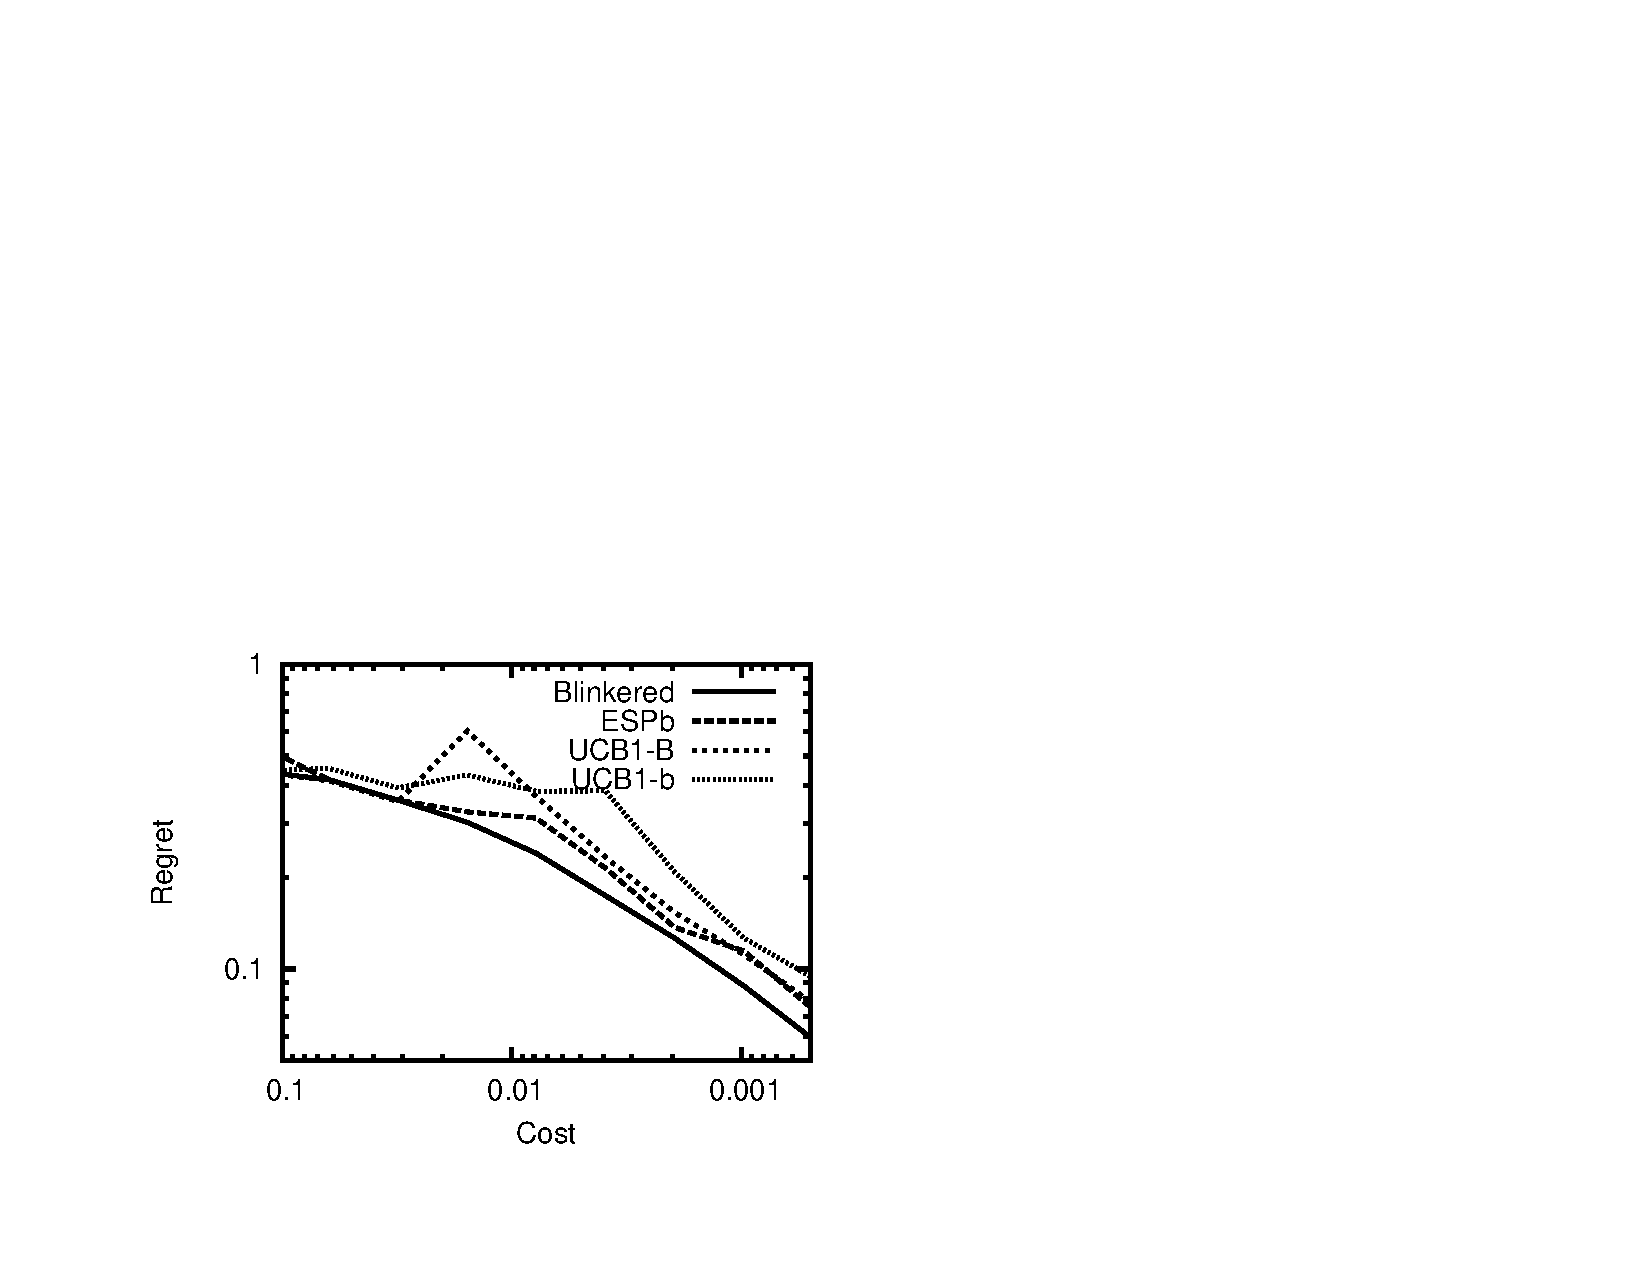
\includegraphics[scale=0.7, trim=90 70 400 300]{blinkered-regret.pdf}
\caption{Regret vs. cost}
\label{fig:blinkered}
\end{figure}

\begin{comment}
set xlabel "Cost"
set ylabel "Regret"

set terminal postscript enhanced linewidth 2
set output "blinkered-regret.ps"
set size 0.5, 0.5

set logscale xy

plot [0.1:0.0005] [0.05:1] "blinkered-regret.dat" title "Blinkered" with lines lw 2, "espb-regret.dat" title "ESPb" with lines lw 2, "ucb-blinkered-regret.dat" title "UCB1-B" with lines lw 2, "ucb-blinkered-table-regret.dat" with lines lw 2 title "UCB1-b"	
\end{comment}
